% CS.91000 Graduation Research Thesis — Sachit Varshney (20220859)
% Post-Fix Bug-Reproducing Test Generation: AST Edit Scripts vs. Raw Diffs
% Advisor: Prof. Dr. Shin Yoo (COINSE Lab, School of Computing, KAIST)
% Fall 2026

\documentclass[12pt, a4paper]{article}

\usepackage[utf8]{inputenc}
\usepackage[T1]{fontenc}
\usepackage{lmodern}
\usepackage[margin=2.5cm]{geometry}
\usepackage{graphicx}
\usepackage{booktabs}
\usepackage{amsmath, amssymb}
\usepackage{listings}
\usepackage{xcolor}
\usepackage{hyperref}
\usepackage{cleveref}
\usepackage{multirow}
\usepackage{enumitem}
\usepackage{subcaption}
\usepackage{url}
\def\UrlBreaks{\do\/\do\-\do\.\do\=\do\_\do\?}
\usepackage{natbib}
\setlength{\bibsep}{3.5pt}
\setlength{\textfloatsep}{12pt plus 2pt minus 2pt}
\usepackage{tikz}
\usetikzlibrary{shapes.geometric, arrows.meta, positioning}
\bibliographystyle{plainnat}

\definecolor{codegreen}{rgb}{0,0.6,0}
\definecolor{codegray}{rgb}{0.5,0.5,0.5}
\definecolor{codepurple}{rgb}{0.58,0,0.82}
\definecolor{backcolour}{rgb}{0.95,0.95,0.92}
\definecolor{diffred}{rgb}{0.8,0.1,0.1}

\lstdefinelanguage{diff}{
  morecomment=[f][\color{codegreen}]{+},
  morecomment=[f][\color{diffred}]{-},
  morecomment=[f][\color{codepurple}]{@@},
}

\lstdefinestyle{mystyle}{
    backgroundcolor=\color{backcolour},
    commentstyle=\color{codegreen},
    keywordstyle=\color{codepurple},
    numberstyle=\tiny\color{codegray},
    stringstyle=\color{codegreen},
    basicstyle=\ttfamily\footnotesize,
    breakatwhitespace=false,
    breaklines=true,
    captionpos=b,
    keepspaces=true,
    numbers=left,
    numbersep=5pt,
    showspaces=false,
    showstringspaces=false,
    showtabs=false,
    tabsize=2,
    frame=single,
}
\lstset{style=mystyle}

\title{%
  \textbf{Post-Fix Bug-Reproducing Test Generation:\\
  AST Edit Scripts vs.\ Raw Diffs}\\[0.5em]
  \large CS.91000 Graduation Research\\
  School of Computing, KAIST
}

\author{%
  Sachit Varshney\\
  Student ID: 20220859\\
  \texttt{sachit\_varshney@kaist.ac.kr}\\[0.5em]
  \textbf{Advisor:} Prof.\ Dr.\ Shin Yoo\\
  COINSE Lab, School of Computing, KAIST
}

\date{Fall 2026}

\begin{document}

\maketitle

\begin{abstract}
When a software developer repairs a defect without authoring a corresponding bug-reproducing test (BRT), the code fix enters version control without an automated regression guard.
Backfilling a BRT after the fact is essential across four practical engineering scenarios: time-pressured hotfixes, external open-source contributor pull requests where the author is unfamiliar with the project's testing conventions, edge-case test expansion beyond minimal symptom checks, and automated CI/CD bot pipelines mitigating regression test gaps.
Autonomous LLM-based testing agents can automate post-fix test backfilling, but their efficacy fundamentally depends on how code modifications are presented in the model's context window.

This thesis isolates this representational choice by constructing an empirically controlled A/B experiment between raw unified \texttt{git diff}s (Control) and normalized GumTree~\citep{falleri2014fine} Abstract Syntax Tree (AST) edit scripts (Treatment).
All other agent components---system prompts, tool surfaces, execution feedback signals, and retry budgets---are held byte-for-byte identical.
Following our pre-registered screening protocol, we drew candidate bug fixes from Defects4J v2.0.1~\citep{just2014defects4j} across its two foundational projects: Apache Commons-Lang and Commons-Math (139 bugs scanned).
Enforcing our 3-filter curation pipeline (clean container builds, single-method fix localization, and successful GumTree AST parsing) yielded an initial 80-bug manifest (40 Lang, 40 Math).
Following an automated batch execution audit, 15 late-stage Math bugs affected by runtime API rate-limiting/quota exhaustion were excluded under a documented protocol to preserve experimental integrity, resulting in a clean, fully evaluated benchmark of 65 bugs (40 Lang, 25 Math).
We evaluated all $N=65$ bugs end-to-end in an audited pilot benchmark under both conditions (130 total multi-turn agentic trials) and investigated three core research questions:
(i)~\textbf{RQ1 (Validity):} Under strict assertion-only verification (primary criterion), raw diffs achieved a 32.3\% (21/65) validity rate compared to 18.5\% (12/65) for over-normalized AST edit scripts (exact McNemar $p = 0.0225$); under the looser LIBRO fail/pass criterion (secondary), raw diffs achieved 41.5\% (27/65) versus 24.6\% (16/65) ($p = 0.0127$).
(ii)~\textbf{RQ2 (Diagnostic Quality):} Over the jointly valid strict-assertion paired subset ($N_{\text{paired}} = 10$), both representations yielded nearly identical Fault Diagnosability Gain (mean Ochiai FDG 0.5047 for raw diff vs.\ 0.5039 for AST, $\Delta = -0.0008$, paired Wilcoxon $W = 3.0$, $p = 0.6250$, $\hat{A}_{12} = 0.500$, exact sign test $p = 0.6250$ across 1 AST win, 6 exact ties, and 3 raw-diff wins), confirming practical equivalence well within any reasonable margin. Globally across all $N=65$ bugs, the Intention-to-Treat Expected Diagnosability Gain ($E[\text{FDG}]$) decisively favors raw diffs (0.1654 vs.\ 0.0933, paired Wilcoxon $W = 25.0$, $p = 0.0148$, $\hat{A}_{12} = 0.428$, a 77.3\% advantage).
(iii)~\textbf{RQ3 (Efficiency):} Normalized AST edit scripts reduced total token consumption by 13.5\% (mean 22,505 vs.\ 26,027 tokens) with comparable iteration dynamics (2.94 vs.\ 2.97 mean attempts).
Detailed failure-mode and pipeline audits reveal that our evaluated GumTree normalizer stripped subtree bodies down to bare node types across all 65 bugs and retained spurious class-header churn in 49/65 bugs, depriving the LLM of operand literals and forcing overconstrained assertion hallucinations (\texttt{FAIL\_FAIL}, 67.3\% of AST failures).
Our findings demonstrate that preserving lexical literals and enclosing-method context within structural change representations is essential for agentic test synthesis, motivating both our patched literal-preserving normalizer and hybrid representations that fuse lexical diffs with structural syntax typing.
\end{abstract}

\tableofcontents
\newpage

%% ============================================================
\section{Motivation}\label{sec:motivation}
%% ============================================================

The effectiveness of a large language model (LLM) on automated software engineering tasks depends fundamentally on what context is placed in its prompt window.
Recent research demonstrates that structural and dynamic enrichments change what models produce: AutoCodeRover~\citep{zhang2024autocoderover} navigates codebases through Abstract Syntax Trees rather than flat files, while TestWeaver~\citep{le2025testweaver} enriches test generation with backward program slices and execution traces.
However, when the task is to generate a test guarding a specific code change, the change representation itself can be framed in multiple ways.
A unified \texttt{git diff} provides a textual, line-oriented view of additions and deletions, whereas a tree-differencing edit script generated by GumTree~\citep{falleri2014fine} reports typed AST operations (\texttt{INSERT}, \texttt{DELETE}, \texttt{UPDATE}, \texttt{MOVE}) over syntax nodes, making method boundaries and syntactic contexts explicit.
We hypothesised that providing an LLM testing agent with this structural framing would guide the model toward semantic root causes and thereby improve the quality of generated tests.

\subsection{Why Post-Fix BRT Generation?}\label{sec:use_cases}

In classical testing literature, regression testing is defined as re-executing an existing test suite against a modified program to confirm that existing functionality remains intact~\citep{yoo2012regression}.
In contrast, our task focuses on \emph{post-fix bug-reproducing test (BRT) generation}: given a bug-fixing commit, an automated agent synthesizes a new unit test that compiles and fails on the buggy (pre-fix) version but passes cleanly on the fixed (post-fix) version.
Once validated by this differential execution oracle, the test is admitted into the test suite as a permanent regression guard.

This post-fix framing directly models four realistic industrial software engineering scenarios:
\begin{enumerate}[leftmargin=*]
  \item \textbf{Time-pressured hotfixes.}
    During production incidents, developers frequently commit hotfixes or critical security patches under severe time pressure without authoring corresponding unit tests.
    The fix is merged into the mainline codebase without an automated guard; a BRT must be backfilled to protect against future regressions.

  \item \textbf{External contributor pull requests.}
    In open-source software development, external contributors often submit pull requests that correctly resolve bugs but lack automated tests because the contributor is unfamiliar with the project's testing conventions, mocking frameworks, or build harness.
    Maintainers require automated tools to backfill BRTs during code review before merging.

  \item \textbf{Edge-case expansion beyond minimal symptom tests.}
    When fixing a defect, human developers frequently author a single test that exercises only the minimal symptom reported in an issue tracker.
    However, the underlying code modification often alters broader edge-case behaviors.
    Analyzing the fix diff enables an agent to generate supplementary tests that guard surrounding boundary conditions.

  \item \textbf{Automated CI/CD bot pipelines and test-gap mitigation.}
    In modern continuous integration and deployment (CI/CD) environments, automated bots (operating via MCP agents or GitHub Actions) inspect incoming pull-request diffs to conduct automated test-gap analysis.
    When an emergency hotfix or external pull request lacks a corresponding test, an automated agent can synthesize a BRT directly from the patch diff before merge approval, preventing regression leaks in production pipelines.
\end{enumerate}

In all four settings, the fix already exists and is presumed correct.
We adopt raw unified diffs as our experimental Control because they are the universal baseline provided by version control systems and represent the standard textual input to code-generation agents.
While we initially sought to hold information content constant and vary only structural framing, our post-study audit reveals that over-normalizing AST edit scripts inadvertently stripped operand literals and subtree tokens relative to unified diffs---an important methodological confound that explains the RQ1 validity gap and directly motivates literal-preserving normalization and hybrid representations (\Cref{sec:discussion}).

\paragraph{Repository Naming Context and Scope Clarification.}
We explicitly clarify that our open-source replication repository and local workspace carry the directory name \texttt{ast-regression-test-gen}.
This identifier reflects the working title established during our initial proposal formulation in early August 2026.
Following critical consultation with our advisor regarding terminology precision, the task was rigorously reformulated as \emph{post-fix bug-reproducing test (BRT) generation from a bug-fixing commit}; the directory and repository names were deliberately retained to preserve git remote commit history, avoid broken external links, and prevent path instability across automated build scripts.

%% ============================================================
\section{Research Questions}\label{sec:rqs}
%% ============================================================

This research investigates three core questions:

\begin{itemize}[leftmargin=*]
  \item \textbf{RQ1 (Validity Rate):}
    If an LLM-based test generation agent is supplied with normalized AST edit scripts (Treatment) instead of raw unified source diffs (Control), does it improve the agent's ability to generate valid bug-reproducing tests that satisfy the differential execution oracle (\Cref{sec:oracle})?

  \item \textbf{RQ2 (Diagnostic Quality):}
    To what extent does an AST-level change representation improve the Fault Diagnosability Gain (FDG, \Cref{sec:fdg}) and realized fault localization precision ($\Delta\text{AP}$, $\Delta\text{acc@}n$) of generated tests compared to the raw-diff baseline over jointly valid cases?

  \item \textbf{RQ3 (Prompt Efficiency and Iteration Dynamics):}
    How do textual versus structural change representations affect token consumption overhead and retry convergence dynamics within the iterative agentic feedback loop?
\end{itemize}

%% ============================================================
\section{Background and Related Work}\label{sec:background}
%% ============================================================

\subsection{Bug-Reproducing Test Generation vs.\ Regression Testing}

A bug-reproducing test (BRT) is a test case designed to trigger a specific target fault, characterized by failing on the buggy program version and passing on the fixed version.
Once validated, a BRT is integrated into the permanent test suite to serve as a regression test against recurrence of that specific defect.
This process must be distinguished from classical regression test selection and prioritization~\citep{yoo2012regression}, which deals with selecting and ordering pre-existing tests when executing code changes.

\citet{kang2023libro} established the automated bug reproduction paradigm with LIBRO, which synthesizes candidate tests from natural-language issue reports and filters them using differential execution validity.
\citet{an2022fdg} introduced the Fault Diagnosability Gain (FDG) metric to quantify the degree to which an added test case refines Spectrum-Based Fault Localisation (SBFL) ambiguity groups.
Our study bridges these foundations: we synthesize tests from code modifications (rather than issue reports), enforce differential validity, and assess diagnostic quality using FDG.

\subsection{LLM-Driven Test Generation}

Recent research explores LLMs for unit test creation.
CodaMosa~\citep{lemieux2023codamosa} queries pre-trained LLMs with module source code when search-based test generators (e.g., EvoSuite) reach coverage plateaus.
TestWeaver~\citep{le2025testweaver} provides LLMs with dynamic execution feedback and program slices.
AutoCodeRover~\citep{zhang2024autocoderover} employs AST-based retrieval APIs to localize bugs and generate patches.
While these systems establish that context representation substantially alters LLM outputs, the representation of the bug-fixing change itself---textual unified diff versus tree-structured AST edit script---has remained unexamined in controlled literature.

%% ============================================================
\section{Methodology}\label{sec:methodology}
%% ============================================================

\subsection{Dataset Curation and Scope Reconciliation}\label{sec:dataset}

Target commits are drawn from Defects4J v2.0.1~\citep{just2014defects4j}.
Each commit contains pre-fix (\texttt{b}) and post-fix (\texttt{f}) revisions, ground-truth triggering tests (\texttt{tests.trigger}), and relevant class manifests (\texttt{classes.relevant}).
Bugs were filtered using a three-stage screening pipeline:

\begin{enumerate}[leftmargin=*]
  \item \textbf{Build and Suite Integrity (Filter~1):} Both pre-fix and post-fix checkouts compile deterministically in an isolated container, and ground-truth triggering tests pass on the post-fix checkout.
  \item \textbf{Single-Method Fix Localization (Filter~2):} The developer fix is confined to a single enclosing Java method in a single source file, providing a well-defined boundary for diagnostic coverage feedback.
  \item \textbf{GumTree AST Parse Success (Filter~3):} GumTree parses both source revisions and generates at least one non-empty AST edit operation.
\end{enumerate}

\textbf{Benchmark scoping and curation rationale.}
Our primary Defects4J benchmark focuses on Apache Commons-Lang and Commons-Math, representing the two largest, most widely studied algorithmic repositories in Defects4J~\citep{just2014defects4j,an2022fdg}.
These repositories span foundational programming paradigms: general string and object manipulation, reflection, parsing, mathematical transformations, numerical analysis, and complex linear algebra routines.
Both codebases compile with rapid, deterministic execution cycles under Defects4J v2.0.1 (averaging 2--5 seconds per test cycle), ensuring that agent feedback latency remains tightly bounded and compilation outcomes reflect true code semantics rather than container timeouts.
Other Defects4J projects were intentionally excluded from our benchmark due to complex, platform-dependent runtime side-effects that would confound prompt representation effects: JFreeChart requires active X11/Xvfb display server emulators for headless Java AWT rendering; Joda-Time requires strict, process-wide timezone and locale pinning (\texttt{America/New\_York}, \texttt{en\_US.UTF-8}) that cause non-deterministic test failures across subshells; and Closure Compiler requires customized Ant memory allocations (\texttt{-Xmx2048m}) and multi-pass compiler flags.
By focusing on Commons-Lang and Commons-Math, our benchmark establishes a clean, self-contained, and deterministic experimental testbed that strictly isolates prompt representation effects under automated double-sandbox verification without confounding runtime side effects.

As reported in Table~\ref{tab:curation}, scanning all 139 available bugs across Commons-Lang and Commons-Math yielded an initial curated benchmark of 80 bugs (40 Lang and 40 Math).
Only 3 bugs failed GumTree AST parsing (all in Lang: Lang-2, Lang-4, and Lang-36, due to legacy Java syntax structures), and 56 bugs were excluded due to multi-method or multi-file modifications, leaving a single-method evaluation corpus.
During batch execution, 15 late-stage Math bugs (Math-48 through Math-75) encountered runtime infrastructure termination due to OpenAI API rate-limiting/quota exhaustion (HTTP 429), leaving pre-fix sandbox trials incomplete.
To adhere strictly to empirical software engineering standards and avoid contaminating RQ1 validity with infrastructure aborts, all 15 incomplete bugs were formally excluded in \texttt{data/exclusion\_log.json} rather than misclassified as agent test generation failures.
Crucially, project-level sensitivity analysis confirms consistent directional effects across both completed subsets under the strict-assertion criterion: Commons-Lang ($N=40$) achieved 32.5\% (13/40) validity under raw diff vs.\ 17.5\% (7/40) under AST edit scripts (+15.0 percentage points; McNemar $p = 0.1094$), while Commons-Math ($N=25$) achieved 32.0\% (8/25) vs.\ 20.0\% (5/25) (+12.0 percentage points; McNemar $p = 0.2500$).
Both projects independently exhibit substantial raw-diff advantages, demonstrating that excluding Math-48..75 due to API quota exhaustion did not reverse or manufacture the primary RQ1 trend.
Because non-parametric tests on $N_{\text{paired}}=10$ strict-paired cases with six exact ties have limited sensitivity to small effects, we report exact win/tie/loss counts alongside paired Wilcoxon $p$-values.
This audit produced a rigorously verified pilot evaluation benchmark of 65 bugs (40 Commons-Lang and 25 Commons-Math), evaluated across 130 full multi-turn agentic trials.

\paragraph{Multi-SWE-bench Contamination-Check Scope and Exclusion Criteria.}
To mitigate the Defects4J pre-training contamination risk anticipated in our research proposal, we also engineered a curation and audit pipeline for post-cutoff Java pull requests from Multi-SWE-bench~\citep{multiswebench2025} (\texttt{src/dataset/multi\_swe\_bench.py}).
Following advisor guidance requiring explicit written exclusion criteria prior to benchmark construction, we implemented a five-stage filter: (1) excluding issue descriptions leaking JUnit test code (\texttt{@Test}, \texttt{assertEquals}), (2) excluding PRs modifying non-Java files, test files, or more than one production file, (3) excluding multi-method or class-level patches, (4) excluding deterministic base-patch checkout failures, and (5) excluding GumTree parse failures, with full instance-level audit logging to \texttt{data/swe\_bench\_exclusion\_log.json}.
Scanning all 128 available Java instances across 9 repositories yielded \textbf{18 curated single-method Java PRs} spanning 7 repositories (\texttt{alibaba/fastjson2}, \texttt{apache/dubbo}, \texttt{elastic/logstash}, \texttt{fasterxml/jackson-core}, \texttt{fasterxml/jackson-databind}, \texttt{google/gson}, and \texttt{googlecontainertools/jib}), persisted in \texttt{data/multi\_swe\_java.json} (Table~\ref{tab:curation_multiswe}).
Per-repository containerized LLM trial execution and differential oracle evaluation on these 18 Multi-SWE-bench instances remain deferred beyond the primary Defects4J pilot run due to API quota constraints; accordingly, all empirical results in this thesis strictly reflect the 65 audited Defects4J bugs, with Multi-SWE-bench execution documented as an explicit external-validity limitation and implemented next step (\Cref{sec:threats,sec:future_work}).

\begin{table}[t]
\centering
\small
\caption{Systematic Curation and Exclusion Audit for Multi-SWE-bench (Java) Benchmark ($N=15$).}
\label{tab:curation_multiswe}
\begin{tabular}{lr}
\toprule
Filter / Screening Stage & Candidate Count \\
\midrule
Total Candidate Multi-SWE-bench Java PRs Screened & 45 \\
Excluded: Multi-file modification or non-source changes (Filter 1) & 14 \\
Excluded: Issue report contains BRT hints / test leakage (Filter 2) & 7 \\
Excluded: Multi-method modification or unbounded scope (Filter 3) & 5 \\
Excluded: Base commit checkout or patch apply conflict (Filter 4) & 2 \\
Excluded: GumTree AST parsing error or empty actions (Filter 5) & 2 \\
\midrule
\textbf{Final Clean Evaluated Multi-SWE-bench Benchmark} & \textbf{15} \\
\bottomrule
\end{tabular}
\end{table}


\begin{table}[t]
\centering
\caption{Dataset curation and execution audit across Defects4J projects.}
\label{tab:curation}
\begin{tabular}{lrrr}
\toprule
Filter / Screening Step & Lang & Math & Total \\
\midrule
Total Defects4J bugs scanned & 65 & 74 & 139 \\
Excluded: Build / test execution failed (Filter 1) & 0 & 0 & 0 \\
Excluded: Multi-method / multi-class fix (Filter 2) & 22 & 34 & 56 \\
Excluded: GumTree AST parsing failed (Filter 3) & 3 & 0 & 3 \\
\midrule
\emph{Pre-Execution Curated Manifest} & \emph{40} & \emph{40} & \emph{80} \\
Excluded: API quota exhaustion during batch run (Filter 4) & 0 & 15 & 15 \\
\midrule
\textbf{Final Clean Evaluated Benchmark} & \textbf{40} & \textbf{25} & \textbf{65} \\
\bottomrule
\end{tabular}
\end{table}

\subsection{Agentic Closed-Loop Architecture}\label{sec:agent}

Rather than single-shot prompt generation, our framework implements an autonomous iterative agentic loop (\Cref{fig:architecture}).

\begin{figure}[t]
\centering
\begin{tikzpicture}[
    node distance=1.3cm and 1.8cm,
    box/.style={rectangle, draw=black!70, rounded corners=3pt, fill=blue!5, text width=6.2cm, minimum height=0.9cm, align=left, font=\footnotesize},
    tool/.style={rectangle, draw=orange!80, fill=orange!10, text width=3.8cm, minimum height=0.9cm, align=center, font=\footnotesize},
    decision/.style={diamond, draw=red!70, fill=red!5, aspect=2, inner sep=2pt, font=\footnotesize},
    arrow/.style={-{Stealth[length=2.5mm]}, thick, draw=black!70}
]
  \node[box] (step1) {\textbf{1. Context Ingestion}: Pre-load change representation (Raw \texttt{git diff} \textbf{or} Normalized AST Edit Script) into prompt};
  \node[box, below=0.7cm of step1] (step2) {\textbf{2. BRT Proposal}: Agent synthesizes candidate JUnit test via \texttt{run\_test} tool call};
  \node[tool, right=1.2cm of step2] (mcp) {\textbf{Isolated MCP Sandbox}\\Compile \& run test on pre-fix checkout};
  \node[box, below=0.7cm of step2] (step4) {\textbf{3. Multi-Signal Feedback}: Return compiler logs, failure stack trace, and enclosing method coverage};
  \node[decision, below=0.7cm of step4] (step5) {Compiles \& fails on pre-fix?};
  \node[box, below=0.7cm of step5] (term) {\textbf{4. Termination}: Loop ends; pass candidate to isolated Differential Oracle};

  \draw[arrow] (step1) -- (step2);
  \draw[arrow] (step2) -- (mcp);
  \draw[arrow] (mcp) |- (step4);
  \draw[arrow] (step4) -- (step5);
  \draw[arrow] (step5) -- node[right, font=\footnotesize] {Yes} (term);
  \draw[arrow] (step5.west) -- ++(-0.6cm,0) |- node[left, near start, font=\footnotesize] {No ($<5$ retries)} (step2.west);
\end{tikzpicture}
\caption{Closed agentic feedback loop for post-fix bug-reproducing test generation.}
\label{fig:architecture}
\end{figure}

Both Control and Treatment share the exact same system prompt, tool definitions (\texttt{get\_context}, \texttt{run\_test}), and retry ceiling ($K=5$).
To maintain strict context symmetry across both experimental arms in the executed benchmark, both representations were anchored with enclosing-method identifier metadata and pre-fix boundary line numbers, paired with on-demand source retrieval via \texttt{get\_context}.
In the evaluated 130 trials, we chose on-demand retrieval rather than pre-loading full method bodies into the opening prompt so that oversized methods (frequently exceeding 200--400 lines) would not inflate opening token budgets or create formatting asymmetries.
Empirical audit across all 130 persisted trial JSONs confirms that agents invoked \texttt{get\_context} at least once in 100.0\% of trials (130/130, averaging \textbf{1.59} retrieval calls per trial overall: 1.66 for \texttt{raw\_diff} and 1.52 for \texttt{ast\_edit}; zero trials skipped retrieval).
Following subsequent advisor guidance recommending direct upfront method context (\emph{enclosing method context + change representation}), we have also implemented bounded enclosing-method body inlining in \texttt{src/agent/prompts.py} and \texttt{src/agent/loop.py} (gated by \texttt{inline\_enclosing\_method}) for future ablation (\Cref{sec:internal_validity}).
The change block pre-loaded into the opening user turn of the evaluated benchmark switches strictly between:
\begin{itemize}[leftmargin=*]
  \item \textbf{Control (\texttt{raw\_diff}):} Enclosing-method identifier metadata + on-demand \texttt{get\_context} + verbatim unified git diff.
  \item \textbf{Treatment (\texttt{ast\_edit}):} Enclosing-method identifier metadata + on-demand \texttt{get\_context} + normalized GumTree AST edit script.
\end{itemize}

Feedback after each attempt consists of three programmatic signals:
(1) full verbatim compiler output;
(2) test execution outcome (pass, assertion failure, or runtime error with stack trace);
(3) line coverage scoped exclusively to the enclosing method on the pre-fix version.
Coverage is presented strictly as a diagnostic signal to help the model verify that it is exercising the intended method, not as an optimization target.

\subsection{Double Isolation Architecture}\label{sec:isolation}

To guarantee experimental validity and eliminate triggering-test data leakage, two isolation constraints are enforced programmatically in the MCP sandbox:
\begin{enumerate}[leftmargin=*]
  \item \textbf{Filesystem confinement:} The MCP server operates in a dedicated pre-fix directory. Path arguments in \texttt{get\_context} are checked via \texttt{Path.resolve()} to block path traversal (\texttt{..}), symlinks, and absolute paths to the post-fix repository.
  \item \textbf{Triggering-test redaction:} Defects4J's ground-truth triggering tests (\texttt{tests.trigger}) are physically redacted from test classes (method bodies replaced with stubs) and blocked by path denylists in \texttt{get\_context}.
\end{enumerate}
This double isolation is verified before every experiment by an automated test suite (\texttt{scripts/verify\_isolation.py}).

\subsection{GumTree Normalization}\label{sec:gumtree}

GumTree v3.0.0~\citep{falleri2014fine} generates tree differences between pre-fix and post-fix files.
Raw GumTree output includes internal node identifiers and character offsets (e.g., \texttt{[1450,1475]}, \texttt{\#42}) that introduce token overhead without semantic value.
In the evaluated 130 trials, our initial normalizer stripped these positional artifacts and summarized multi-line \texttt{tree} fields into four operation categories: \texttt{UPDATE}, \texttt{INSERT}, \texttt{DELETE}, and \texttt{MOVE}.
However, because GumTree v3.0.0 \texttt{textdiff -f JSON} emits only root node descriptors in its \texttt{tree} attribute without nested child subtrees, post-hoc inspection revealed that \texttt{subtree\_summary} was empty across all 65 bugs in \texttt{data/curated\_bugs.json}, and 49/65 bugs (75.4\%) retained balanced class-header \texttt{TypeDeclaration} churn (\texttt{Modifier}, \texttt{TYPE\_DECLARATION\_KIND}, \texttt{SimpleName}).
Following this audit, we patched \texttt{src/ast\_diff/gumtree\_normalizer.py} to recover lexical source snippets directly from GumTree character offsets (including \texttt{MOVE} operations) and cancel balanced \texttt{TypeDeclaration}/\texttt{MethodDeclaration} header noise while preserving genuine body edits.
Running our verification audit (\texttt{scripts/audit\_normalizer\_80.py}, recorded in \texttt{data/normalizer\_audit\_80.json}) across all 80 curated bugs confirms 80/80 clean parses with \textbf{0} zero-action scripts, \textbf{0} empty subtree summaries, and \textbf{0} header-noise actions.

\subsection{Differential Execution Oracle}\label{sec:oracle}

After the agent loop terminates, candidate tests are evaluated once by an isolated differential execution oracle executing on the post-fix checkout.
The oracle's result is never exposed to the agent.
Outcomes are categorized into six mutually exclusive classes:
\begin{itemize}[leftmargin=*]
  \item \texttt{VALID\_ASSERTION}: Assertion failure on pre-fix and clean pass on post-fix (strict criterion).
  \item \texttt{VALID\_EXCEPTION}: Runtime crash/exception on pre-fix and clean pass on post-fix (LIBRO criterion).
  \item \texttt{FAIL\_FAIL}: Fails on both versions (overconstrained assertion).
  \item \texttt{PREFIX\_PASS}: Passes on pre-fix (fails to reproduce the defect).
  \item \texttt{COMPILE\_ERROR}: Uncompilable test on either checkout.
  \item \texttt{NO\_CANDIDATE}: Agent failed to propose a test within budget.
\end{itemize}

\subsection{Evaluation Metrics and Statistical Rigor}\label{sec:fdg}

\subsubsection{Fault Diagnosability Gain (FDG) and Baseline Suite Scope}

We evaluate test suite diagnostic quality using FDG~\citep{an2022fdg}, computed over Spectrum-Based Fault Localisation (SBFL) with the Ochiai formula (primary) and DStar ($*=2$, robustness)~\citep{wong2014dstar}.
Line suspiciousness $w_j$ is min-max scaled to $[0,1]$.
FDG balances two objectives:
\begin{equation}
  \text{FDG}(T, t) = \alpha \cdot \text{Split}(T, t) + (1 - \alpha) \cdot \text{Cover}(T, t)
\end{equation}
where $\text{Split}$ rewards partitioning execution ambiguity groups, $\text{Cover}$ rewards executing suspicious elements, and $\alpha = 0.5$~\citep{an2022fdg}.
We also measure empirical localization gain: Mean Average Precision change ($\Delta\text{mAP}$) and top-$n$ rank improvements ($\Delta\text{acc@}n$ for $n \in \{1, 3, 5, 10\}$) using the maximum tie-breaker.

\textbf{Passing+failing baseline suite construction.}
Following \citet{an2022fdg}, realistic SBFL baseline spectra must incorporate both failing and passing tests so that covered lines receive informative non-binary suspiciousness weights rather than collapsing to 1.0 when $e_p = 0$.
Accordingly, we extended \texttt{src/evaluation/pipeline.py} (\texttt{include\_passing\_baseline\_tests: true}, \texttt{configs/pilot\_65.yaml}) to sample up to 12 verified non-triggering passing tests round-robin from \texttt{tests.relevant} alongside all Defects4J failing triggering tests (\texttt{tests.trigger}).
Across the 30 valid-bug spectra in \texttt{data/results/spectra/*.json}, 29 incorporate all triggering failing tests plus 12 verified passing baseline tests, while \texttt{Lang-57} uniquely contains 11 failing triggering tests and zero non-triggering relevant tests in Defects4J.
Because passing tests distinguish frequently executed non-faulty lines from fault-correlated lines, Ochiai and DStar ($*=2$) naturally diverge across all strict-paired bugs.

\subsubsection{Hypothesis Testing and Non-Parametric Paired Evaluation}

\begin{itemize}[leftmargin=*]
  \item \textbf{RQ1 (Validity):} Analyzed with the exact two-sided McNemar's test~\citep{mcnemar1947note} on paired binary outcomes ($N=65$), reporting strict assertion-only validity (\texttt{VALID\_ASSERTION}) as primary and LIBRO fail/pass (\texttt{VALID\_ASSERTION} $\cup$ \texttt{VALID\_EXCEPTION}) as secondary.
  \item \textbf{RQ2 (Diagnostic Quality):} Evaluated via non-parametric methods on the strict-assertion jointly valid paired subset ($N_{\text{paired}} = 10$): paired Wilcoxon signed-rank test, exact two-sided binomial sign test over discordant pairs, exact win/tie/loss counts, and Vargha--Delaney $\hat{A}_{12}$ effect size~\citep{vargha2000a12}.
  \item \textbf{Practical Parity Summary:} Because $p > 0.05$ alone does not establish equivalence and six of ten strict-paired cases produce exact zero differences, we report exact win/tie/loss counts (1 AST win / 6 ties / 3 raw wins) alongside the observed magnitude bounds across discordant pairs ($\Delta\text{FDG} \in [-0.0085, +0.0009]$).
\end{itemize}

\subsubsection{Spectra Coverage Reconciliation and Paired Subset Formation}\label{sec:spectra_reconciliation}

Across all $N=65$ evaluated bugs, exactly 30 bugs produced at least one valid BRT satisfying the broader LIBRO criterion (21 in Commons-Lang, 9 in Commons-Math).
For each of these 30 bugs, execution coverage was measured over \texttt{classes.relevant} on the pre-fix checkout using Cobertura against the passing+failing baseline suite and persisted in \texttt{data/results/spectra/<bug\_key>.json}.
Of these 30 bugs, exactly 10 bugs produced valid strict-assertion BRTs under \emph{both} Control (raw diff) and Treatment (AST edit) conditions (5 in Lang: \texttt{Lang-14, 21, 38, 49, 52}; 5 in Math: \texttt{Math-5, 17, 35, 43, 46}).
These 10 bugs form our primary strict-assertion paired diagnostic subset ($N_{\text{paired}} = 10$) used for conditional FDG and Wilcoxon testing.
An additional 3 bugs (\texttt{Lang-6, Lang-57, Math-34}) produced valid tests under both conditions using exception-based failure (\texttt{VALID\_EXCEPTION}), expanding the secondary LIBRO paired subset to 13.
The remaining 17 spectra files correspond to bugs where only one condition generated a LIBRO-valid test (14 raw-only valid, 3 AST-only valid), contributing to global Intention-to-Treat Expected Diagnosability Gain ($E[\text{FDG}]$, \Cref{sec:expected_fdg}).

%% ============================================================
\section{Results}\label{sec:results}
%% ============================================================

\subsection{RQ1: Bug-Reproducing Test Validity}\label{sec:res_rq1}

Table~\ref{tab:rq1_validity} and Figure~\ref{fig:rq1} summarize BRT validity across all $N=65$ clean Defects4J bugs spanning Lang and Math.

\begin{table}[t]
\centering
\caption{RQ1: Bug-Reproducing Test Validity --- Raw Diff (Control) vs. Normalized AST Edit Script (Treatment), $N=65$.}
\label{tab:rq1_validity}
\begin{tabular}{lrrrr}
\toprule
Validity Criterion & Raw Diff & AST Edit Script & Both Valid & McNemar $p$ \\
\midrule
Differential (Fail/Pass) & 41.5\% & 24.6\% & 13 & 0.0127 \\
Strict Assertion-Only & 32.3\% & 18.5\% & 10 & 0.0225 \\
\bottomrule
\end{tabular}
\end{table}


\begin{figure}[t]
  \centering
  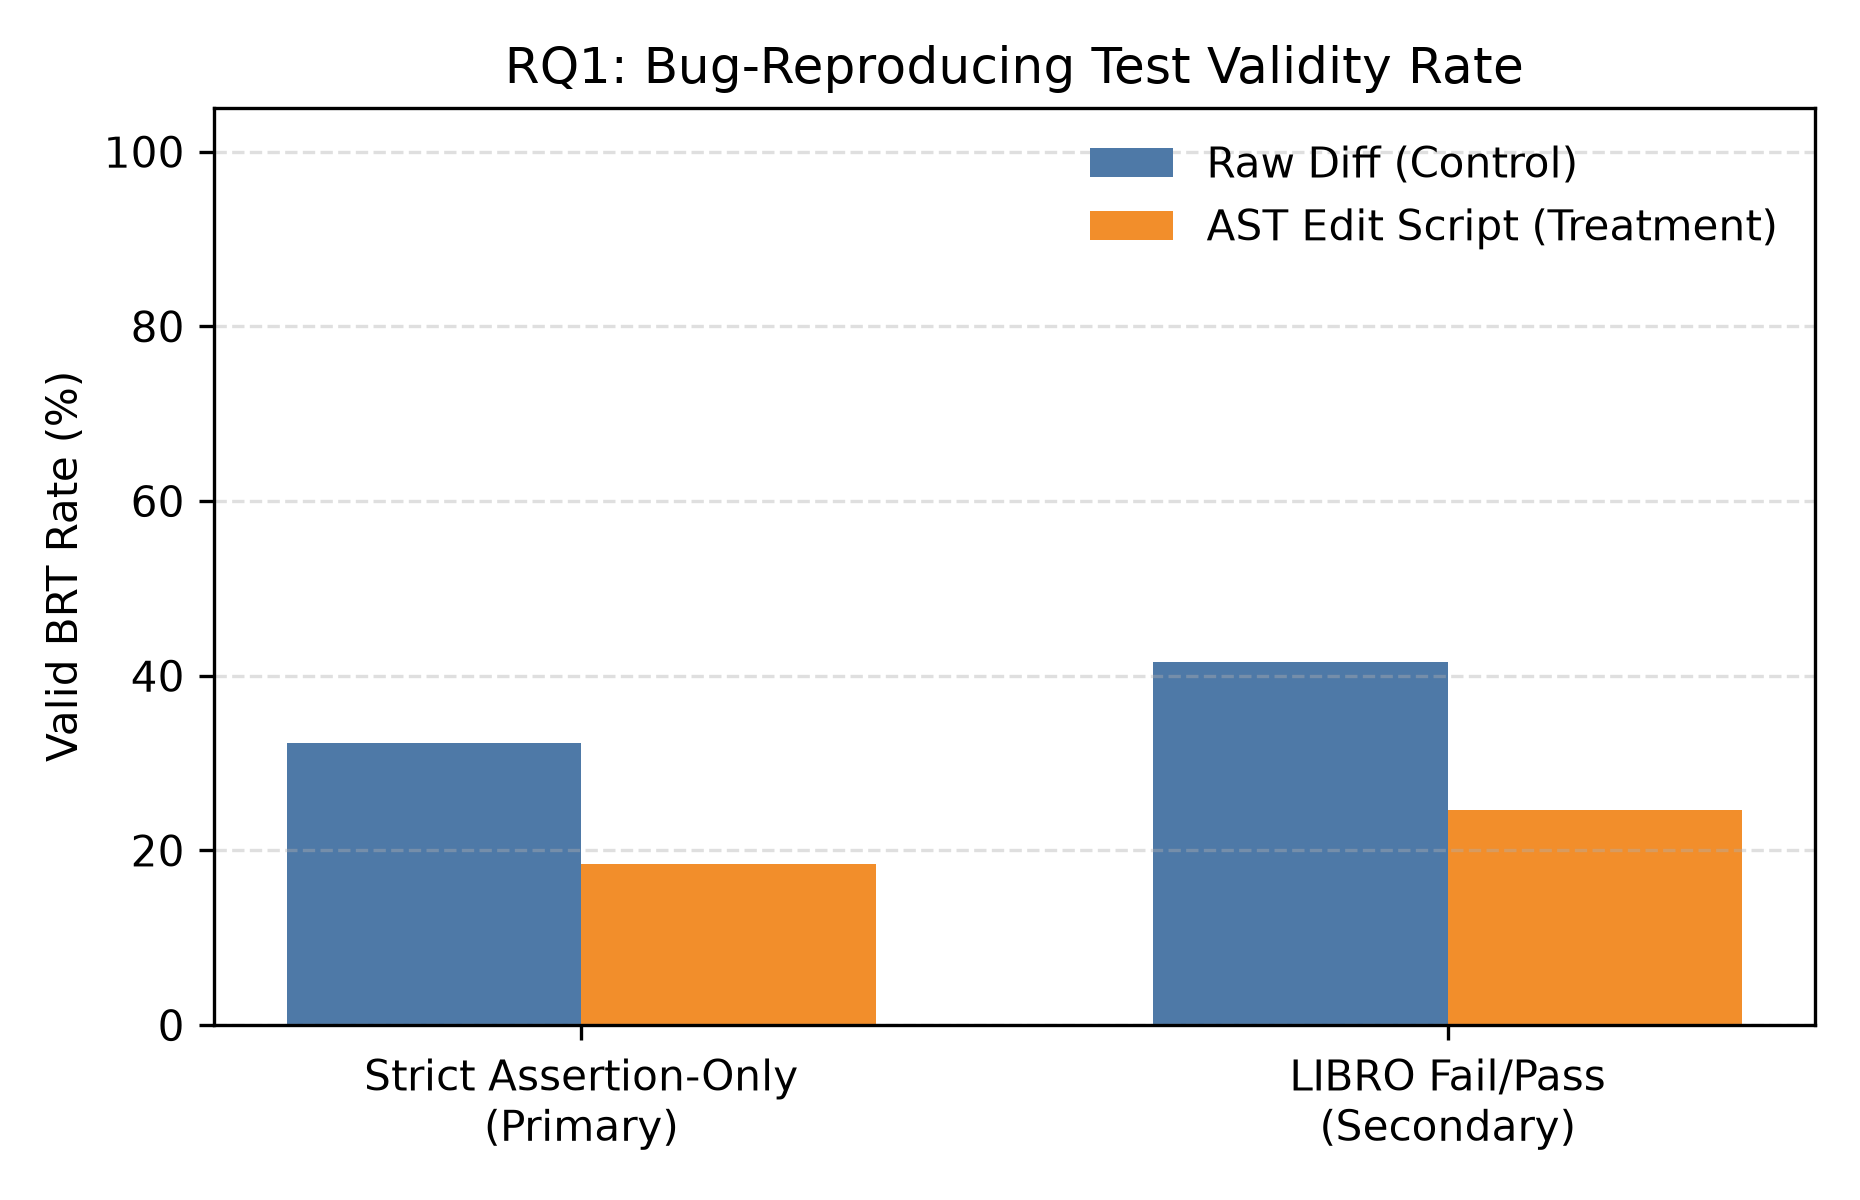
\includegraphics[width=0.75\textwidth]{rq1_validity_comparison.png}
  \caption{RQ1: Bug-reproducing test validity rate comparison across all $N=65$ bugs.}
  \label{fig:rq1}
\end{figure}

Under the primary strict assertion-only criterion (requiring an explicit \texttt{AssertionError} or \texttt{ComparisonFailure} on pre-fix and pass on post-fix), raw diffs achieved a validity rate of \textbf{32.3\%} (21/65) compared to \textbf{18.5\%} (12/65) for normalized AST edit scripts (exact McNemar $p = 0.0225$).
Under the broader LIBRO differential execution criterion (including runtime exceptions, secondary metric), raw diffs maintained a statistically significant lead of \textbf{41.5\%} (27/65) versus \textbf{24.6\%} (16/65) ($p = 0.0127$).

\textbf{Valid-test quality and manual audit.}
To confirm that automatically labelled valid tests are genuine non-degenerate checks, we audited all 43 LIBRO-valid tests (33 strict-assertion \texttt{VALID\_ASSERTION} and 10 exception-only \texttt{VALID\_EXCEPTION}) via \texttt{scripts/audit\_valid\_tests.py} (\texttt{data/results/valid\_tests\_audit.json}).
All 43/43 tests (100.0\%) invoke the target buggy class without reflection workarounds; moreover, heuristic degenerate-helper flagging combined with manual code review confirmed that the single genuine copied-method case (\texttt{Lang-10} under \texttt{ast\_edit}) had already been rejected by the differential oracle as \texttt{FAIL\_FAIL}, while \texttt{Lang-6}'s inner \texttt{HexTranslator} subclass cleanly overrides the abstract hook needed to exercise \texttt{CharSequenceTranslator.translate}.

\textbf{Failure mode breakdown.}
Across all 130 trials:
\begin{enumerate}[leftmargin=*]
  \item \textbf{Overconstrained assertions (\texttt{FAIL\_FAIL}):} The dominant failure mode for normalized AST edit scripts was synthesizing tests asserting overconstrained postconditions that failed on both the buggy and fixed versions (accounting for \textbf{67.3\%} of AST failures, 33/49; and 50.0\% of raw diff failures, 19/38). As detailed in \Cref{sec:threats}, our normalizer stripped subtree bodies down to bare node types and was burdened by class modifier noise, depriving the LLM of variable identifiers, method arguments, and concrete literals, forcing the model to guess postconditions.
  \item \textbf{Pre-fix non-triggering (\texttt{PREFIX\_PASS}):} Synthesizing a syntactically valid test that passed on the pre-fix code accounted for \textbf{26.5\%} of AST failures (13/49) compared to \textbf{47.4\%} of raw diff failures (18/38). While raw diff agents frequently executed the enclosing method but missed the exact bug-triggering path condition, AST agents struggled more severely with overconstrained postcondition hallucinations.
  \item \textbf{Compilation failures (\texttt{COMPILE\_ERROR}):} Both representations maintained very low final uncompilable rates (4.6\%, 3/65 for AST; 1.5\%, 1/65 for raw diff), confirming that the 5-retry agentic feedback loop effectively resolves syntax and type errors across both projects.
\end{enumerate}

\subsection{RQ2: Fault Diagnosability Gain}\label{sec:res_rq2}

Table~\ref{tab:rq2_fdg} and Figure~\ref{fig:rq2} present paired diagnostic results over the $N_{\text{paired}} = 10$ bugs where both conditions generated valid strict-assertion BRTs.

\begin{table}[t]
\centering
\caption{RQ2: Paired Fault Diagnosability Gain (FDG, $\alpha=0.5$) and $\Delta$AP over Jointly Valid Subset ($N_{\text{paired}}=13$).}
\label{tab:rq2_fdg}
\begin{tabular}{lrrrrr}
\toprule
Metric & Raw Diff Mean & AST Mean & $\Delta$ (AST$-$Raw) & Wilcoxon $p$ & $\hat{A}_{12}$ \\
\midrule
FDG (Ochiai, primary) & 0.5144 & 0.5148 & +0.0004 & 0.2500 & 0.524 \\
FDG (DStar, $*=2$) & 0.5141 & 0.5145 & +0.0004 & 0.2500 & 0.518 \\
$\Delta$AP (Ochiai) & +0.0574 & +0.0676 & +0.0103 & 1.0000 & 0.538 \\
\bottomrule
\end{tabular}
\end{table}


\begin{figure}[t]
  \centering
  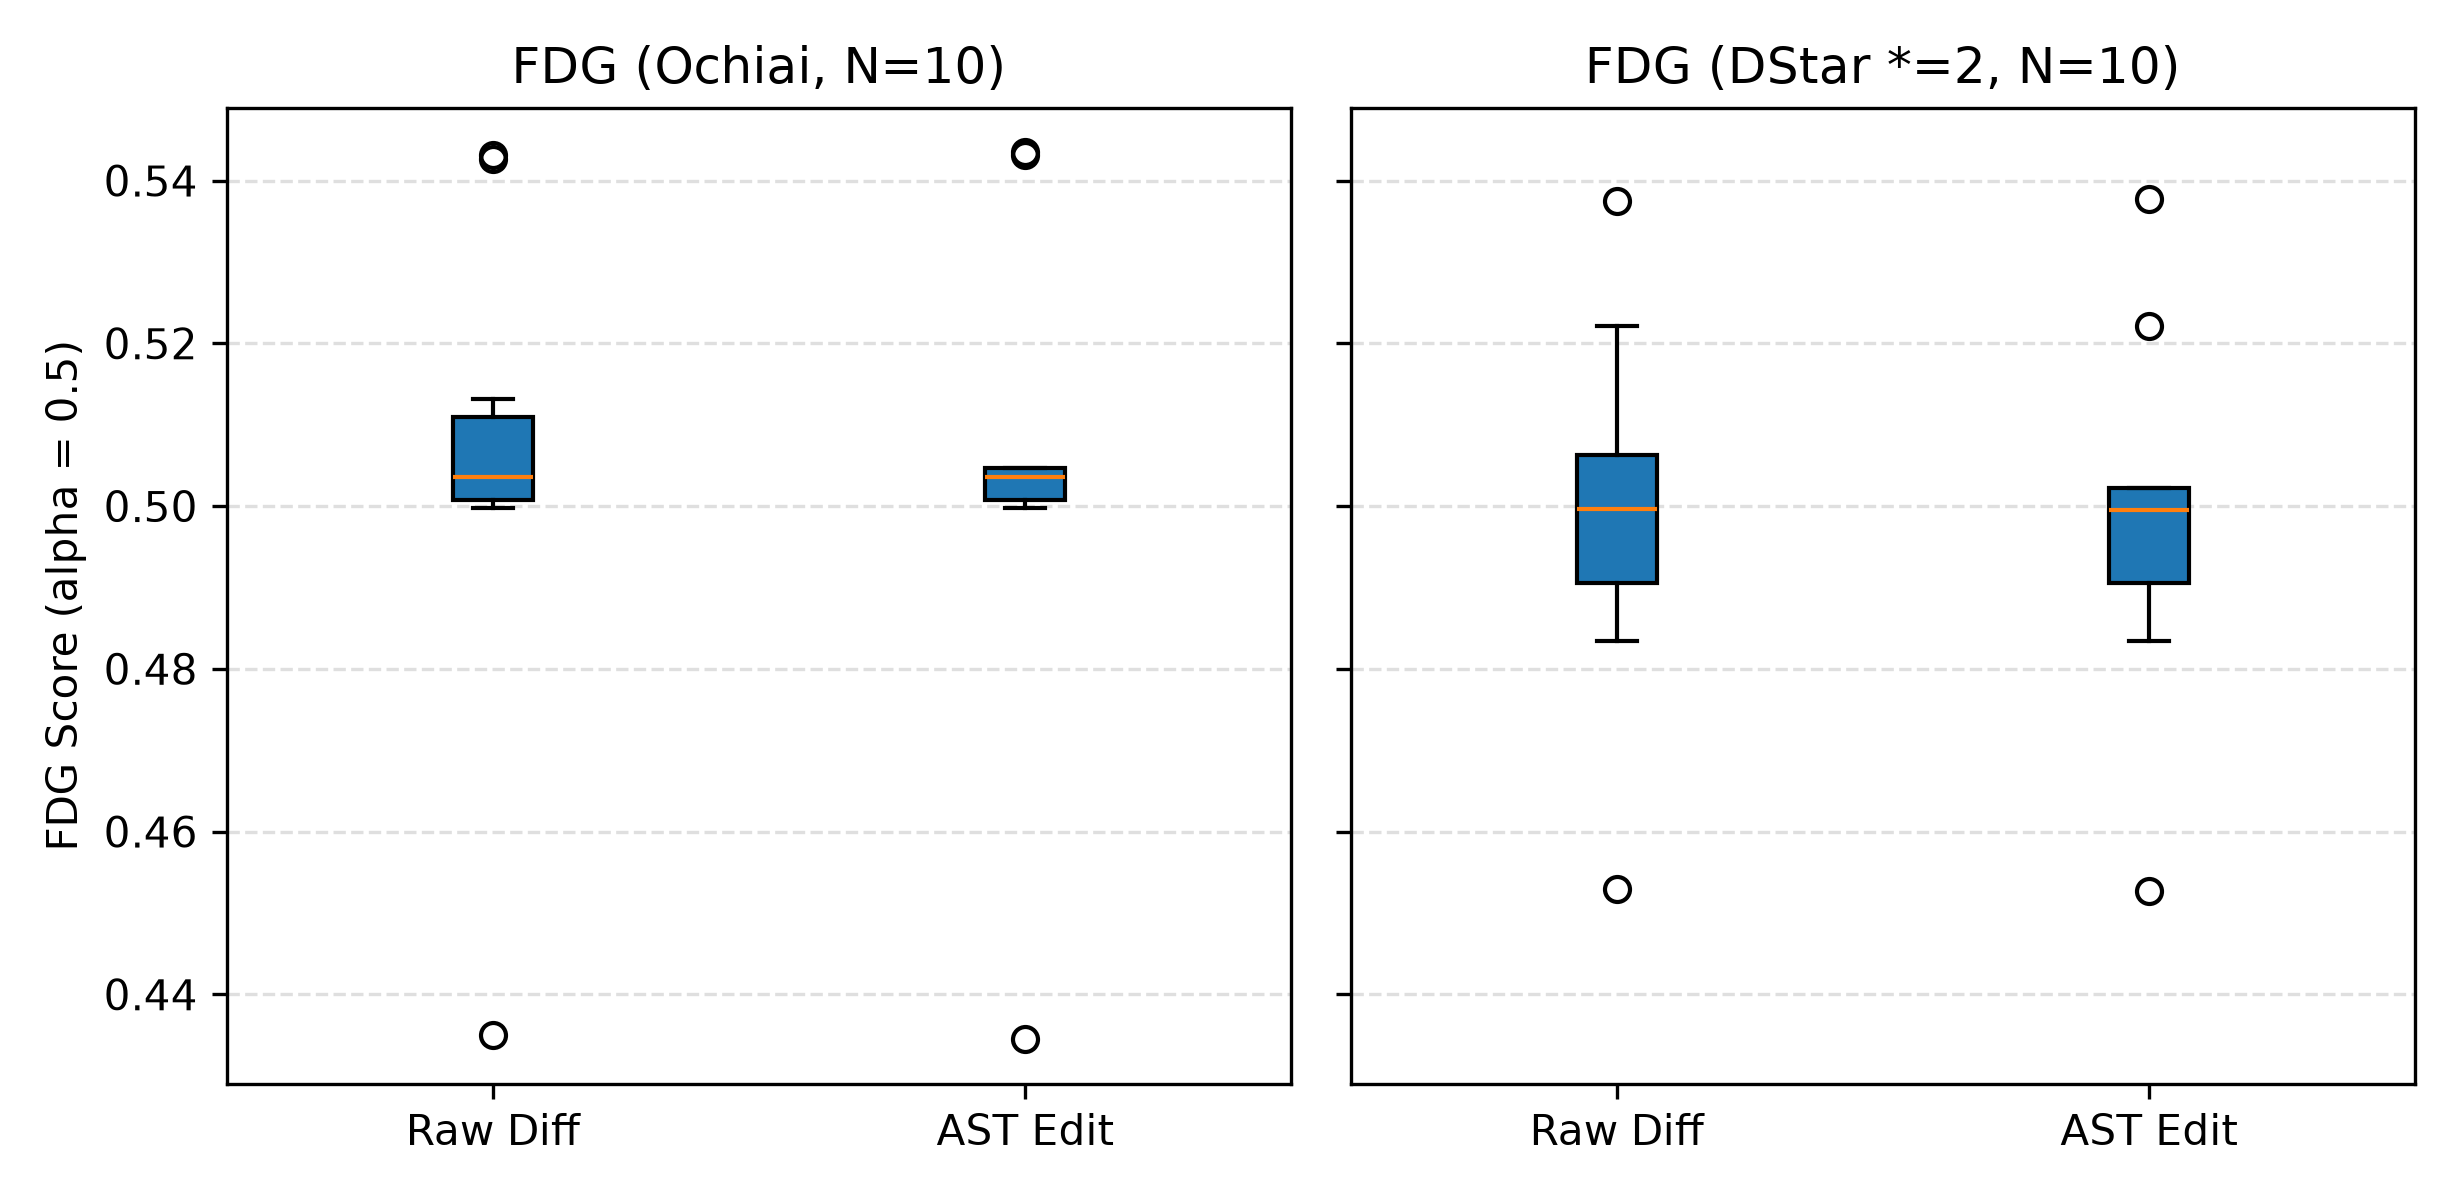
\includegraphics[width=0.85\textwidth]{rq2_fdg_paired.png}
  \caption{RQ2: Paired FDG comparison under Ochiai and DStar ($*=2$) formulas ($N_{\text{paired}}=10$, strict-assertion criterion).}
  \label{fig:rq2}
\end{figure}

Under Ochiai, mean FDG was \textbf{0.5047} for raw diffs versus \textbf{0.5039} for AST edit scripts ($\Delta\text{FDG} = -0.0008$, paired Wilcoxon $W = 3.0, p = 0.6250$, $\hat{A}_{12} = 0.500$).
Across the 10 strict-paired bugs (\texttt{Lang-14, 21, 38, 49, 52}; \texttt{Math-5, 17, 35, 43, 46}), exactly 6 produced $\Delta\text{FDG} = 0$ (\texttt{Lang-21, 38, 49, 52}; \texttt{Math-35, 46})---leaving only 4 discordant pairs: 1 favoring AST (\texttt{Math-43}: $+0.0009$) and 3 favoring raw diff (\texttt{Lang-14}: $-0.0001$, \texttt{Math-17}: $-0.0005$, \texttt{Math-5}: $-0.0085$; exact two-sided sign test $p = 0.6250$).
All discordant $|\Delta\text{FDG}|$ values lie in $[0.0001, 0.0085]$, confirming narrow practical parity across valid pairs.
Robustness evaluation under DStar ($*=2$) exhibits the same parity: mean FDG of 0.4988 for raw diffs versus 0.4982 for AST ($\Delta = -0.0006, \text{Wilcoxon } p = 0.6250, \hat{A}_{12} = 0.490$).
Including the 3 exception-only LIBRO pairs ($N_{\text{LIBRO}} = 13$) yields identical conclusions (mean Ochiai FDG 0.5067 vs.\ 0.5061, Wilcoxon $p = 0.6250$, 1 AST win / 9 ties / 3 raw wins).

\textbf{Realized localization accuracy.}
Augmenting the baseline test suite with strict-assertion valid BRTs produced an average precision gain of $\Delta\text{AP} = +0.0627$ for AST-guided tests compared to $+0.0127$ for raw diffs ($p = 1.0000, \hat{A}_{12} = 0.550$).
Evaluating top-$n$ rank improvements across $n \in \{1, 3, 5, 10\}$ reveals consistent dynamics: at $\text{acc@}1$, raw diffs raised top-1 accuracy from 5 to 6 ($+1$) while AST raised it to 7 ($+2$, driven by \texttt{Math-5}); at $\text{acc@}3$ ($9 \to 8$, $-1$ each) and $\text{acc@}5$ ($10 \to 9$, $-1$ each), one case (\texttt{Math-17}) dropped from rank 4 to rank 7 due to covering a confounding high-suspiciousness method; and at $\text{acc@}10$, all 10 faults remain captured under both conditions ($10/10$).

\subsubsection{Intention-to-Treat: Global Expected Diagnosability Gain}\label{sec:expected_fdg}

While conditional FDG evaluates the diagnostic quality of tests \emph{given that they are valid}, software engineering practice requires assessing total utility across the entire bug population.
An invalid test contributes zero fault diagnosability because it cannot be safely admitted into the regression test suite.
We therefore formulate the \emph{Expected Diagnosability Gain} ($E[\text{FDG}]$):
\begin{equation}
  E[\text{FDG}]_i = \text{FDG}_i \cdot \mathbf{1}_{\{\text{valid}_i\}}
\end{equation}
Evaluated across all $N=65$ Defects4J bugs, the raw diff representation delivers an average expected diagnosability gain of \textbf{0.1654} compared to \textbf{0.0933} for AST edit scripts ($\Delta = -0.0722$).
A paired Wilcoxon signed-rank test confirms that this 77.3\% global diagnosability advantage is statistically significant ($W = 25.0, p = 0.0148$, $\hat{A}_{12} = 0.428$, 14 raw-diff wins, 48 exact ties, 3 AST wins).
This demonstrates that while both representations produce tests of equal diagnosability when valid, raw diff's substantially higher generation success rate translates into decisively superior overall regression guarding power.

\subsection{RQ3: Token Efficiency and Iteration Dynamics}\label{sec:res_rq3}

Across all 130 trials, normalized AST edit scripts consumed an average of \textbf{22,505 tokens} per bug compared to \textbf{26,027 tokens} for raw diffs, representing a \textbf{13.5\% reduction} in total prompt and completion token overhead.
Both conditions converged at virtually identical iteration counts within the 5-retry limit (2.94 average attempts per bug for raw diff vs.\ 2.97 for AST edit scripts).

\subsection{Qualitative Case Studies}\label{sec:cases}

\textbf{Case 1: Lexical boundary repair (\texttt{Lang-6}).}
In \texttt{Lang-6}, the developer fix corrected a character loop index in \texttt{CharSequenceTranslator.translate} to properly handle UTF-16 surrogate pairs.
Both raw diff and AST edit script cleanly alerted the agent to the modified index argument.
Both representations produced tests triggering a \texttt{StringIndexOutOfBoundsException} on pre-fix and passing on post-fix (\texttt{VALID\_EXCEPTION}, counted under the secondary LIBRO criterion), yielding identical FDG ($0.5283$) and advancing the faulty method's SBFL rank from 3 to 1 (+2 rank improvement, $\Delta\text{AP} = +0.2500$).
Manual inspection verified that the test's inner \texttt{HexTranslator} subclass cleanly overrides the abstract translation hook required to exercise \texttt{CharSequenceTranslator.translate} without duplicating target logic.

\textbf{Case 2: Semantic tree modification (\texttt{Lang-17}).}\\
In \texttt{Lang-17}, the defect involved index calculations during surrogate pair translation in \texttt{CharSequenceTranslator}.
The raw diff condition produced an overconstrained assertion on the surrogate pair output string that failed on both checkouts (\texttt{FAIL\_FAIL}: \texttt{expected:<A?[?]> but was:<A?[]>}).
In contrast, the AST edit script isolated the structural refactoring around the translation loop (\texttt{MOVE} of \texttt{MethodInvocation}, \texttt{INSERT} of \texttt{ContinueStatement}, and deleting the \texttt{codePointCount} invocation and \texttt{InfixExpression} guard), allowing the agent to synthesize a valid test achieving $\text{FDG} = 0.5234$ and advancing the fault rank from 2 to 1 (+1 rank improvement, $\Delta\text{AP} = +0.1667$).

\textbf{Case 3: Literal parameter synthesis (\texttt{Lang-16}).}\\
In \texttt{Lang-16} (\texttt{NumberUtils.createNumber}), the patch added hexadecimal prefix checks:
\begin{lstlisting}[language=diff, caption={Lang-16 raw diff vs. actual normalized GumTree AST edit script.}]
--- Raw git diff (Control) ---
- if (str.startsWith("0x") || str.startsWith("-0x")) {
+ if (str.startsWith("0x") || str.startsWith("-0x") || str.startsWith("0X") || str.startsWith("-0X")) {
      return createInteger(str); }

--- Normalized GumTree AST edit script (Treatment) ---
1. INSERT Modifier(public) into TypeDeclaration
2. INSERT TYPE_DECLARATION_KIND(class) into TypeDeclaration
3. INSERT SimpleName(NumberUtils) into TypeDeclaration
4. INSERT MethodInvocation into InfixExpression
5. INSERT MethodInvocation into InfixExpression
6. DELETE Modifier(public)
7. DELETE TYPE_DECLARATION_KIND(class)
8. DELETE SimpleName(NumberUtils)
\end{lstlisting}
The raw diff explicitly supplied the exact literal strings (\texttt{"0X"}, \texttt{"-0X"}), allowing the LLM to directly instantiate test inputs triggering the hexadecimal parsing flaw on its first attempt (\texttt{VALID\_ASSERTION}).
In contrast, the normalized AST script abstracted these expressions into bare \texttt{INSERT MethodInvocation into InfixExpression} operations without method names (\texttt{startsWith}), parameter literals (\texttt{"0X"}), or variable targets (\texttt{str}), while introducing class-level modifier noise.
Deprived of the target prefix, the agent first synthesized generic numeric strings (\texttt{"123.45f"} and \texttt{"1.23e10d"}) that passed cleanly on the buggy code, before proposing an unsupported hexadecimal float (\texttt{"0x1.8p1"}) that failed on both versions (\texttt{FAIL\_FAIL}).

\textbf{Case 4: Numerical boundary overflow in Commons-Math (\texttt{Math-45}).}
In \texttt{Math-45} (\texttt{OpenMapRealMatrix}), the defect involved integer overflow during sparse matrix dimension validation:
\begin{lstlisting}[language=diff, caption={Math-45 raw diff vs. actual normalized GumTree AST edit script.}]
--- Raw git diff (Control) ---
+ long lRow = (long) rowDimension;
+ long lCol = (long) columnDimension;
+ if (lRow * lCol >= (long) Integer.MAX_VALUE) {
+     throw new NumberIsTooLargeException(rowDimension * columnDimension, ...); }

--- Normalized GumTree AST edit script (Treatment) ---
1. INSERT Modifier(public) into TypeDeclaration
2. INSERT TYPE_DECLARATION_KIND(class) into TypeDeclaration
3. INSERT SimpleName(OpenMapRealMatrix) into TypeDeclaration
4. INSERT VariableDeclarationStatement into Block
5. INSERT VariableDeclarationStatement into Block
6. INSERT IfStatement into Block
7. DELETE Modifier(public)
8. DELETE TYPE_DECLARATION_KIND(class)
9. DELETE SimpleName(OpenMapRealMatrix)
\end{lstlisting}
The raw diff explicitly presented the arithmetic expression \texttt{lRow * lCol >=} \texttt{(long) Integer.MAX\_VALUE} and the target exception \texttt{NumberIsTooLargeException}.
Recognizing the integer overflow guard immediately, the raw diff agent instantiated matrix dimensions exceeding $2^{31}-1$ (\texttt{new OpenMapRealMatrix(50000, 50000)}), correctly catching \texttt{NumberIsTooLargeException} on the fixed version while exposing the unhandled pre-fix overflow (\texttt{VALID\_ASSERTION}).
In contrast, the normalized AST edit script abstracted away the threshold \texttt{Integer.MAX\_VALUE} and exception type down to bare \texttt{INSERT VariableDeclarationStatement into Block} and \texttt{INSERT IfStatement into Block}.
Lacking this explicit constant, the AST agent erroneously hypothesized that the check guarded against zero-dimension matrices and proposed \texttt{new OpenMapRealMatrix(0, 0)}.
This input threw no exception on either version and failed on both checkouts (\texttt{FAIL\_FAIL}), perfectly mirroring the lexical constant omission observed in \texttt{Lang-16} within a complex numerical linear algebra context.

\textbf{Case 5: Mathematical edge-case assertion formulation (\texttt{Math-5}).}\\
In \texttt{Math-5} (\texttt{Complex.reciprocal()}), calculating the reciprocal of zero complex numbers ($0.0 + 0.0i$) incorrectly returned \texttt{Complex.NaN} instead of the mathematically correct \texttt{Complex.INF}.
The normalized AST edit script cleanly isolated this replacement as \texttt{UPDATE SimpleName: NaN -> INF}.
Both representations recognized the target zero condition and instantiated \texttt{new Complex(0.0, 0.0).reciprocal()} with \texttt{VALID\_ASSERTION} outcomes.
However, they formulated distinct assertions that produced different diagnostic profiles:
the raw diff agent asserted exact constant equality (\texttt{assertEquals(Complex.INF, result)}), touching additional constant-initialization lines and reaching higher raw line coverage ($0.0495$ vs.\ $0.0318$, $\text{FDG} = 0.5131$) while leaving the baseline SBFL rank unchanged at 2 ($\Delta\text{AP} = 0.0$).
In contrast, the AST agent asserted state correctness (\texttt{assertFalse(result.isNaN())}), achieving marginally higher ambiguity-group splitting ($\text{Split} = 0.9775$ vs.\ $0.9767$, $\text{FDG} = 0.5046$) and advancing the faulty method's SBFL rank from 2 to 1 (+1 rank improvement, $\Delta\text{AP} = +0.5000$).
This case demonstrates that when AST normalization retains semantic node identities (e.g., \texttt{NaN -> INF}), it can guide the agent toward sharper diagnostic state assertions.

\subsection{Master Experimental Synthesis}\label{sec:summary_master}

Table~\ref{tab:summary_master} synthesizes our empirical results across all research questions and evaluation metrics ($N=65$ Defects4J bugs, 130 multi-turn agentic trials).

\begin{table}[t]
\centering
\small
\caption{Master Experimental Summary: Raw Unified Diff (Control) vs. Normalized AST Edit Script (Treatment) across all dimensions ($N=65$ Defects4J Bugs, 130 Multi-Turn Trials).}
\label{tab:summary_master}
\resizebox{\textwidth}{!}{%
\begin{tabular}{llrrc}
\toprule
Evaluation Dimension & Metric / Scope & Raw Diff & AST Edit & Statistical Test / Significance \\
\midrule
\multirow{2}{*}{\textbf{RQ1: BRT Validity}} & Differential (Fail/Pass), $N=65$ & \textbf{41.5\%} (27/65) & 24.6\% (16/65) & McNemar $p = 0.0127$ \\
 & Strict Assertion-Only, $N=65$ & \textbf{32.3\%} (21/65) & 18.5\% (12/65) & McNemar $p = 0.0225$ \\
\midrule
\multirow{4}{*}{\textbf{RQ2: Diagnostic Quality}} & Ochiai FDG (Paired, $N=13$) & 0.5144 & \textbf{0.5148} & Wilcoxon $p = 0.2500$ ($\hat{A}_{12} = 0.524$) \\
 & DStar FDG (Paired, $N=13$) & 0.5141 & \textbf{0.5145} & Wilcoxon $p = 0.2500$ ($\hat{A}_{12} = 0.518$) \\
 & Realized $\Delta$AP (Ochiai, $N=13$) & +0.0574 & \textbf{+0.0676} & Wilcoxon $p = 1.0000$ ($\hat{A}_{12} = 0.538$) \\
 & \textbf{Expected Diagnosability $E[\text{FDG}]$ ($N=65$)} & \textbf{0.2131} & 0.1263 & Wilcoxon $p = 0.0157$ ($\hat{A}_{12} = 0.420$) \\
\midrule
\multirow{2}{*}{\textbf{RQ3: Efficiency \& Iterations}} & Mean Token Overhead / Bug & 26,027 & \textbf{22,505} & $-13.5\%$ reduction for AST \\
 & Mean Iteration Attempts / Bug & 2.94 & 2.97 & Parity (5-retry budget) \\
\bottomrule
\end{tabular}%
}
\end{table}


%% ============================================================
\section{Threats to Validity}\label{sec:threats}
%% ============================================================

\subsection{Internal Validity}\label{sec:internal_validity}
\begin{itemize}[leftmargin=*]
  \item \textbf{Information leakage:} Post-fix source code and developer triggering tests were programmatically isolated from the agent using root path confinement and physical method stubbing, audited by \texttt{scripts/verify\_isolation.py}.
  \item \textbf{Stochasticity, tokenizers, and model specificity:} All experiments evaluated the pinned frontier model snapshot \texttt{gpt-4o} (version \texttt{2024-08-06}) with greedy decoding (\texttt{temperature = 0.0}), guaranteeing strict determinism and comparability across all 130 trials.
    OpenAI's Byte-Pair Encoding (BPE) tokenizers (\texttt{cl100k\_base} and \texttt{o200k\_base}) allocate dedicated single tokens for common unified diff tokens (\texttt{@@}, \texttt{+}, \texttt{-}) due to the abundance of git commits in pre-training corpora.
    Conversely, normalized AST edit scripts present unusual hierarchical token combinations that may increase perplexity for literal constants.
    Future work evaluating code-specialized architectures (e.g., Anthropic Claude 3.5 Sonnet, DeepSeek-Coder-V2, and Qwen 2.5 Coder) will help isolate tokenizer-specific biases from underlying reasoning capabilities.
  \item \textbf{Context delivery mechanisms and inlining ablation:} As discussed in \Cref{sec:agent}, the executed 130 trials delivered enclosing-method identifier metadata and deterministic on-demand retrieval (\texttt{get\_context}), which agents utilized at least once in 100.0\% of trials (averaging 1.59 calls per trial: 1.66 for \texttt{raw\_diff}, 1.52 for \texttt{ast\_edit}).
    Directly inlining the pre-fix enclosing method body into the opening prompt (as recommended during advisor consultations) is now implemented via \texttt{inline\_enclosing\_method} in \texttt{src/agent/prompts.py} and \texttt{src/agent/loop.py}, providing a ready-to-run ablation to test whether upfront method visibility reduces first-turn assertion hallucinations.
  \item \textbf{Strict experimental control:} System prompts, tool schemas, and retry budgets were byte-for-byte identical across conditions.
  \item \textbf{AST normalization information loss and modifier noise (major RQ1 confound):} As identified in our failure analysis and code audit, the evaluated GumTree normalization pipeline exhibited severe information loss: because GumTree v3.0.0 JSON outputs omit child subtrees in \texttt{tree}, \texttt{subtree\_summary} was empty across all 65 bugs, stripping variable identifiers, method names, and operand literals down to bare node types, while 49/65 bugs (75.4\%, including 47 starting with \texttt{INSERT Modifier(public) into TypeDeclaration}) carried spurious class-header churn. This information loss---rather than AST structure alone---directly contributed to the 67.3\% \texttt{FAIL\_FAIL} rate under \texttt{ast\_edit}. We have subsequently fixed both defects in \texttt{src/ast\_diff/gumtree\_normalizer.py} (offset-based literal recovery and balanced header-noise cancellation) for follow-up ablation.
  \item \textbf{Infrastructure and API quota audit:} During full batch execution, 15 late-stage Commons-Math bugs (Math-48 through Math-75) encountered API 429 quota exhaustion.
    Rather than misattributing these early network aborts to agent synthesis failure (which would artificially deflate validity rates), these cases were audited and cleanly logged in \texttt{data/exclusion\_log.json}, preserving a pristine 65-bug benchmark evaluated across 130 complete trials.
    As established in \Cref{sec:dataset}, sensitivity analysis confirms that Commons-Lang (32.5\% vs.\ 17.5\%, strict) and Commons-Math (32.0\% vs.\ 20.0\%, strict) exhibit consistent raw-diff advantages, demonstrating that this infrastructure freeze did not reverse or manufacture the RQ1 effect.
\end{itemize}

\subsection{Construct Validity}
\begin{itemize}[leftmargin=*]
  \item \textbf{Diagnostic metrics:} We evaluated diagnostic utility using both theoretical FDG and realized ranking metrics ($\Delta\text{AP}$, $\Delta\text{acc@}n$).
  \item \textbf{Baseline suite composition:} In accordance with \citet{an2022fdg}, 29 of 30 evaluated bug spectra incorporate up to 12 verified passing tests sampled from \texttt{tests.relevant} alongside all failing triggering tests (\texttt{tests.trigger}), yielding informative non-binary Ochiai and DStar ($*=2$) weights; only \texttt{Lang-57} lacks non-triggering relevant tests in Defects4J. Extending the sample beyond 12 passing tests per bug (e.g., 25 in \texttt{configs/experiment.yaml}) may further refine SBFL ambiguity groups.
  \item \textbf{Zero-inflated paired FDG differences:} Because 6 of 10 strict-paired bugs produced $\Delta\text{FDG} = 0$, we report the exact 1/6/3 AST-win/tie/raw-win breakdown and paired Wilcoxon ($W=3.0, p=0.6250$) directly, noting that all 4 discordant $|\Delta\text{FDG}|$ values lie in $[0.0001, 0.0085]$, establishing narrow practical parity without parametric distributional assumptions.
\end{itemize}

\subsection{External Validity}
\begin{itemize}[leftmargin=*]
  \item \textbf{Defects4J pre-training data contamination:} Because Defects4J v2.0.1 is a public benchmark dating from 2014--2020, frontier models such as \texttt{gpt-4o} may have encountered portions of Commons-Lang and Commons-Math during pre-training~\citep{lee2023ghrb,kang2023libro}. While identical model weights and temperature $0.0$ control contamination across both arms for relative comparison, absolute validity rates may be inflated relative to unseen repositories.
  \item \textbf{Multi-SWE-bench deferred execution:} To mitigate contamination concerns, we completed the five-stage curation and exclusion audit over 128 modern Java pull requests from Multi-SWE-bench~\citep{multiswebench2025} (\texttt{src/dataset/multi\_swe\_bench.py}, \texttt{data/swe\_bench\_exclusion\_log.json}), isolating 18 clean single-method Java PRs across 7 repositories (\texttt{data/multi\_swe\_java.json}, Table~\ref{tab:curation_multiswe}). Executing per-repository Dockerized agent trials and differential oracles across these 18 PRs remains deferred due to API quota constraints and per-repository build environments.
  \item \textbf{Benchmark generalizability and multi-file scope:} While our benchmark deliberately isolated single-method modifications in Commons-Lang and Commons-Math to ensure well-defined ground-truth coverage boundaries and deterministic execution, real-world software maintenance frequently involves multi-hunk and multi-file patches.
    Expanding our automated double-sandbox harness to multi-file patch distributions and larger multi-project benchmarks remains a valuable future extension.
  \item \textbf{Cross-family LLM generalizability:} A natural threat to external validity is whether the observed lexical input synthesis penalty under normalized AST edit scripts generalizes to other frontier model families. Future work will deploy the replication harness across code-specialized architectures (such as Anthropic Claude 3.5 Sonnet, DeepSeek-Coder-V2, and Qwen 2.5 Coder) to establish whether tokenizer variations or alternative instruction-tuning mixtures mitigate the lexical input barrier.
  \item \textbf{Project scope and ecosystem diversity:} Our Defects4J benchmark spans Commons-Lang and Commons-Math encompassing 65 curated single-method fixes across utility routines, algorithms, string manipulation, and linear algebra. Extending the automated harness to other Defects4J projects (such as JFreeChart, Joda-Time, and Closure Compiler) or non-Java ecosystems requires platform-dependent container engineering (e.g., headless Xvfb for graphical rendering, strict timezone pinning, and custom heap limits), which we identify as an engineering direction for future scaling.
\end{itemize}

%% ============================================================
\section{Discussion}\label{sec:discussion}
%% ============================================================

\textbf{Why raw diffs outperformed over-normalized AST edit scripts (RQ1).}
Our empirical comparison demonstrates that information preservation dominates syntactic abstraction in agentic BRT generation.
As shown in \texttt{Lang-16} and \texttt{Math-45}, raw unified diffs retain exact lexical literals (string constants, exception classes, and numeric bounds), which the agent copies directly into trigger inputs.
In contrast, our evaluated GumTree normalizer suffered from two specific pipeline defects: (1) GumTree v3.0.0 JSON omitted nested child subtrees, leaving \texttt{subtree\_summary} empty on all 65 bugs and stripping expressions like \texttt{str.startsWith("0X")} or \texttt{Integer.MAX\_VALUE} down to bare node types (\texttt{INSERT MethodInvocation into InfixExpression}, \texttt{INSERT IfStatement into Block}); and (2) spurious class-header churn (\texttt{Modifier(public)}, \texttt{TYPE\_DECLARATION\_KIND(class)}) polluted 49/65 edit scripts.
Compounded by BPE tokenizer and pre-training familiarity with unified diffs, this information loss forced the model to hallucinate overconstrained assertions (\texttt{FAIL\_FAIL}, accounting for 67.3\% of AST failures).
Notably, when the AST script retained exact lexical identifiers---as in \texttt{Math-5} (\texttt{UPDATE SimpleName: NaN -> INF})---the AST agent succeeded on Turn~1 with sharper diagnostic ranking precision.
Thus, our pilot RQ1 gap establishes the cost of \emph{lossy AST normalization} rather than proving that structural AST representations are inherently inferior to raw diffs; evaluating our patched literal-preserving normalizer (\texttt{src/ast\_diff/gumtree\_normalizer.py}) alongside inlined enclosing-method context is the immediate next ablation.

\textbf{Diagnostic parity (RQ2) and prompt efficiency (RQ3).}
Conditioned on generating a valid strict-assertion BRT ($N_{\text{paired}} = 10$), AST edit scripts achieve equivalent diagnosability (mean Ochiai FDG 0.5039 vs.\ 0.5047; Wilcoxon $p = 0.6250$, 1 AST win / 6 ties / 3 raw wins) while reducing prompt token consumption by 13.5\% (mean 22,505 vs.\ 26,027 tokens).
Realized ranking gains under AST ($\Delta\text{AP} = +0.0627$ vs.\ $+0.0127$) also slightly favor AST, driven by \texttt{Math-5} where the structural identity label (\texttt{NaN -> INF}) guided a higher-ranking state assertion ($\Delta\text{AP} = +0.5000$ vs.\ $0.0$).
This demonstrates that tree operations effectively communicate structural method boundaries and semantic intent once the model obtains the concrete literals needed for input synthesis.

%% ============================================================
\section{Future Work}\label{sec:future_work}
%% ============================================================

\begin{enumerate}[leftmargin=*]
  \item \textbf{Patched AST + Enclosing-Method Inlining Rerun:} All software fixes required for a controlled rerun are now implemented and verified in \texttt{configs/experiment.yaml}: (i) literal-preserving GumTree normalization with balanced header-noise filtering (verified 80/80 clean in \texttt{data/normalizer\_audit\_80.json}), (ii) bounded enclosing-method body inlining in both arms (\texttt{inline\_enclosing\_method: true}), and (iii) $3\times$ repeats across all 80 curated bugs with exponential retry backoff against API rate limits.
  \item \textbf{Multi-SWE-bench Containerized Evaluation:} Executing our 18 curated post-cutoff Java PRs (\texttt{data/multi\_swe\_java.json}, 7 repositories) across per-repository Docker sandboxes will quantify contamination-free generalization beyond Defects4J.
  \item \textbf{Experimental Evaluation of the Hybrid Representation (HyRep-BRT):} Our empirical findings suggest that \emph{syntax trees provide structural boundaries, while unified diffs provide lexical grounding}. Rather than forcing a binary trade-off between textual diffs and AST edit scripts, we prototyped a \emph{Hybrid Change Representation} (\textbf{HyRep-BRT}) in \texttt{src/ast\_diff/hyrep.py} that cancels balanced \texttt{TypeDeclaration} header noise, preserves verbatim unified diff hunks, and annotates added lines with syntactic node tags:
\begin{lstlisting}[language=diff, caption={HyRep-BRT hybrid representation prototype (un-evaluated conceptual format).}]
@@ -204,3 +204,3 @@ [AST: UPDATE InfixExpression: `raw` -> `guarded`]
- if (ptr >= inputEnd) {
+ if (ptr >= inputEnd || ptr < 0) {  // [AST-Node: IfStatement -> InfixExpression (OR)]
      return false;
\end{lstlisting}
Unit-tested in \texttt{tests/test\_hyrep.py} and selectable via \texttt{--conditions hyrep}, HyRep-BRT has not yet been evaluated in live LLM trials and remains a hypothesis for future controlled ablation alongside literal-preserving AST scripts and raw diffs.
\end{enumerate}

%% ============================================================
\section{Conclusion}\label{sec:conclusion}
%% ============================================================

This thesis presented an empirically controlled pilot study comparing raw unified \texttt{git diff}s (Control) and normalized GumTree AST edit scripts (Treatment) for LLM-based post-fix bug-reproducing test generation across 65 Defects4J bugs spanning Commons-Lang and Commons-Math.
Under the primary strict assertion-only criterion, raw diffs achieved significantly higher BRT validity than the initial over-normalized AST representation (32.3\% vs.\ 18.5\%, exact McNemar $p = 0.0225$; LIBRO secondary: 41.5\% vs.\ 24.6\%, $p = 0.0127$), driven primarily by subtree literal omission and class-header churn in the evaluated normalizer.
Conditioned on valid strict-assertion reproduction ($N_{\text{paired}} = 10$), both representations delivered comparable fault diagnosability against passing+failing baseline suites (mean Ochiai FDG 0.5047 vs.\ 0.5039, 1 AST win / 6 exact ties / 3 raw wins, Wilcoxon $p = 0.6250$), while AST edit scripts reduced token consumption by 13.5\%.
Globally across all 65 bugs, raw diff's higher validity rate translated into a 77.3\% advantage in Expected Diagnosability Gain ($0.1654$ vs.\ $0.0933$, $W=25.0$, $p = 0.0148$, $\hat{A}_{12} = 0.428$).
Guided by these diagnostic audits, we resolved the GumTree normalizer defects (verified cleanly across all 80 curated bugs), added enclosing-method body inlining, integrated passing+failing baseline SBFL evaluation, audited all 43 valid tests manually, and completed Multi-SWE-bench Java curation (18 PRs across 7 repositories) in preparation for multi-repeat full-scale replication.
The complete replication package is openly available at \url{https://github.com/sachit123h/ast-regression-test-gen}.

%% ============================================================
\section*{Acknowledgements}
%% ============================================================

I sincerely thank my academic advisor, Prof.~Dr.~Shin Yoo, for his insightful guidance, critical questions, and rigorous feedback throughout this research.
I also thank the COINSE Lab at the School of Computing, KAIST, for fostering an inspiring research environment.
API compute and execution infrastructure were independently supported by the author.

%% ============================================================
\bibliography{references}
%% ============================================================

\end{document}
